% Options for packages loaded elsewhere
\PassOptionsToPackage{unicode}{hyperref}
\PassOptionsToPackage{hyphens}{url}
%
\documentclass[
]{article}
\usepackage{amsmath,amssymb}
\usepackage{lmodern}
\usepackage{iftex}
\ifPDFTeX
  \usepackage[T1]{fontenc}
  \usepackage[utf8]{inputenc}
  \usepackage{textcomp} % provide euro and other symbols
\else % if luatex or xetex
  \usepackage{unicode-math}
  \defaultfontfeatures{Scale=MatchLowercase}
  \defaultfontfeatures[\rmfamily]{Ligatures=TeX,Scale=1}
  \setmainfont{Noto Serif CJK SC}
  \setsansfont{DejaVu Sans}
  \setmonofont{DejaVu Sans Mono}
  \IfFileExists{xeCJK.sty}{%
    \usepackage{xeCJK}
    \setCJKmainfont{Noto Serif CJK SC}
    \setCJKsansfont{Noto Sans CJK SC}
  }{}
  \IfFileExists{ucharclasses.sty}{%
    \usepackage{ucharclasses}
    \newfontfamily\CJKfont{Noto Serif CJK SC}[BoldFont={Noto Serif CJK SC Bold}]
    \setTransitionsForCJK{\CJKfont}{\rmfamily}
  }{}
\fi
% Use upquote if available, for straight quotes in verbatim environments
\IfFileExists{upquote.sty}{\usepackage{upquote}}{}
\IfFileExists{microtype.sty}{% use microtype if available
  \usepackage[]{microtype}
  \UseMicrotypeSet[protrusion]{basicmath} % disable protrusion for tt fonts
}{}
\makeatletter
\@ifundefined{KOMAClassName}{% if non-KOMA class
  \IfFileExists{parskip.sty}{%
    \usepackage{parskip}
  }{% else
    \setlength{\parindent}{0pt}
    \setlength{\parskip}{6pt plus 2pt minus 1pt}}
}{% if KOMA class
  \KOMAoptions{parskip=half}}
\makeatother
\usepackage{xcolor}
\IfFileExists{xurl.sty}{\usepackage{xurl}}{} % add URL line breaks if available
\IfFileExists{bookmark.sty}{\usepackage{bookmark}}{\usepackage{hyperref}}
\hypersetup{
  hidelinks,
  pdfcreator={LaTeX via pandoc}}
\urlstyle{same} % disable monospaced font for URLs
\usepackage{longtable,booktabs,array}
\usepackage{calc} % for calculating minipage widths
% Correct order of tables after \paragraph or \subparagraph
\usepackage{etoolbox}
\makeatletter
\patchcmd\longtable{\par}{\if@noskipsec\mbox{}\fi\par}{}{}
\makeatother
% Allow footnotes in longtable head/foot
\IfFileExists{footnotehyper.sty}{\usepackage{footnotehyper}}{\usepackage{footnote}}
\makesavenoteenv{longtable}
\usepackage{graphicx}
\makeatletter
\def\maxwidth{\ifdim\Gin@nat@width>\linewidth\linewidth\else\Gin@nat@width\fi}
\def\maxheight{\ifdim\Gin@nat@height>\textheight\textheight\else\Gin@nat@height\fi}
\makeatother
% Scale images if necessary, so that they will not overflow the page
% margins by default, and it is still possible to overwrite the defaults
% using explicit options in \includegraphics[width, height, ...]{}
\setkeys{Gin}{width=\maxwidth,height=\maxheight,keepaspectratio}
% Set default figure placement to htbp
\makeatletter
\def\fps@figure{htbp}
\makeatother
\usepackage[normalem]{ulem}
% Avoid problems with \sout in headers with hyperref
\pdfstringdefDisableCommands{\renewcommand{\sout}{}}
\setlength{\emergencystretch}{3em} % prevent overfull lines
\providecommand{\tightlist}{%
  \setlength{\itemsep}{0pt}\setlength{\parskip}{0pt}}
\setcounter{secnumdepth}{-\maxdimen} % remove section numbering
\ifLuaTeX
  \usepackage{selnolig}  % disable illegal ligatures
\fi

\author{}
\date{}

% Redline macros generated by make_redline.py.
% Deleted text is red struck-through; added text is blue.
\providecommand{\DIFadd}[1]{{\begingroup\color{blue}#1\endgroup}}
\providecommand{\DIFdel}[1]{{\begingroup\color{red}\sout{#1}\endgroup}}

\begin{document}

\textbf{Supporting Information for}

\textbf{Agentic analysis of droplet-engineered appendix-derived gut organoid growth, differentiation, and fusion using AAPS}

\emph{Zhengyu Wu\textsuperscript{1, 3}, Rongzhou Chen \textsuperscript{2,3}, Wanlong Wang\textsuperscript{1}, Chuqian Ruan\textsuperscript{1}, Haotian Sun\textsuperscript{1}, Edmund Y. Lam\textsuperscript{2}, Shaohua Ma\textsuperscript{1,4}}

\begin{enumerate}
\def\labelenumi{\arabic{enumi}.}
\item
  Institute of Biopharmaceutical and Health Engineering (iBHE), Tsinghua Shenzhen International Graduate School (SIGS), Tsinghua University, Shenzhen 518055, China
\item
  Department of Electrical and Computer Engineering, University of Hong Kong, Pokfulam, Hong Kong SAR, China
\item
  These authors contributed equally
\item
  Corresponding Email: ma.shaohua@sz.tsinghua.edu.cn
\end{enumerate}

\textbf{This PDF file contains 4 main items including:}

\begin{quote}
Figures S1 to S3

Tables S1
\end{quote}

\textbf{And:}

\begin{quote}
Legends for Source Data-1,2,3,4,5,6

SI References
\end{quote}

\textbf{Other supporting materials for this manuscript include the following:}

\begin{quote}
Source Data-1

Source Data-2

Source Data-3

Source Data-4

Source Data-5

Source Data-6
\end{quote}

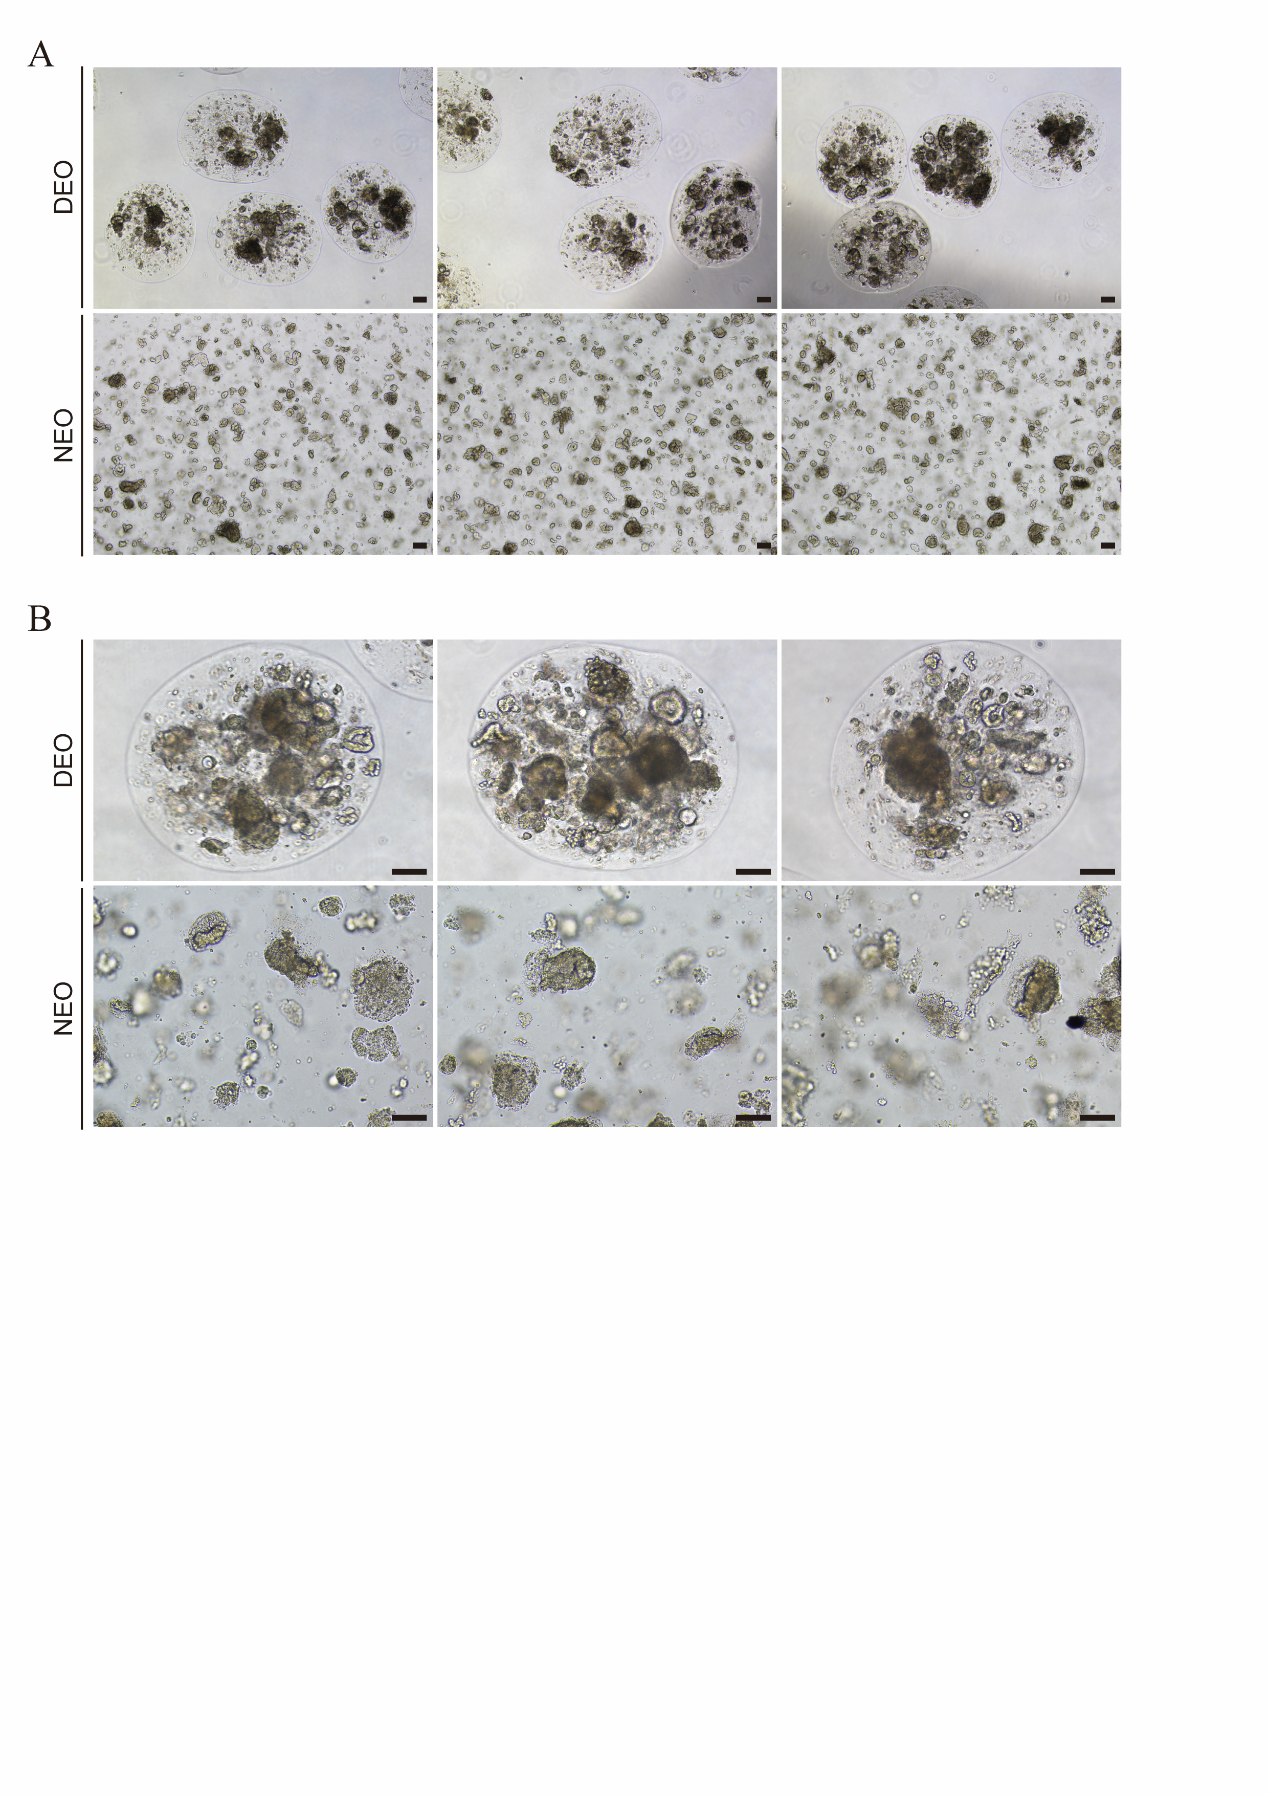
\includegraphics[width=5.13542in,height=5.19792in]{figures/sm_figure_01.png}

Figure S1 The comparisons between droplet-engineered organoid (DEO) and nonengineered organoid (NEO). Representative brightfield images of Day 0 seeding as crypts in Matrigel domes. Images were captured by using 4× objective lenses (A) and 10× objective lenses (B). Scale bars are 100 μm.

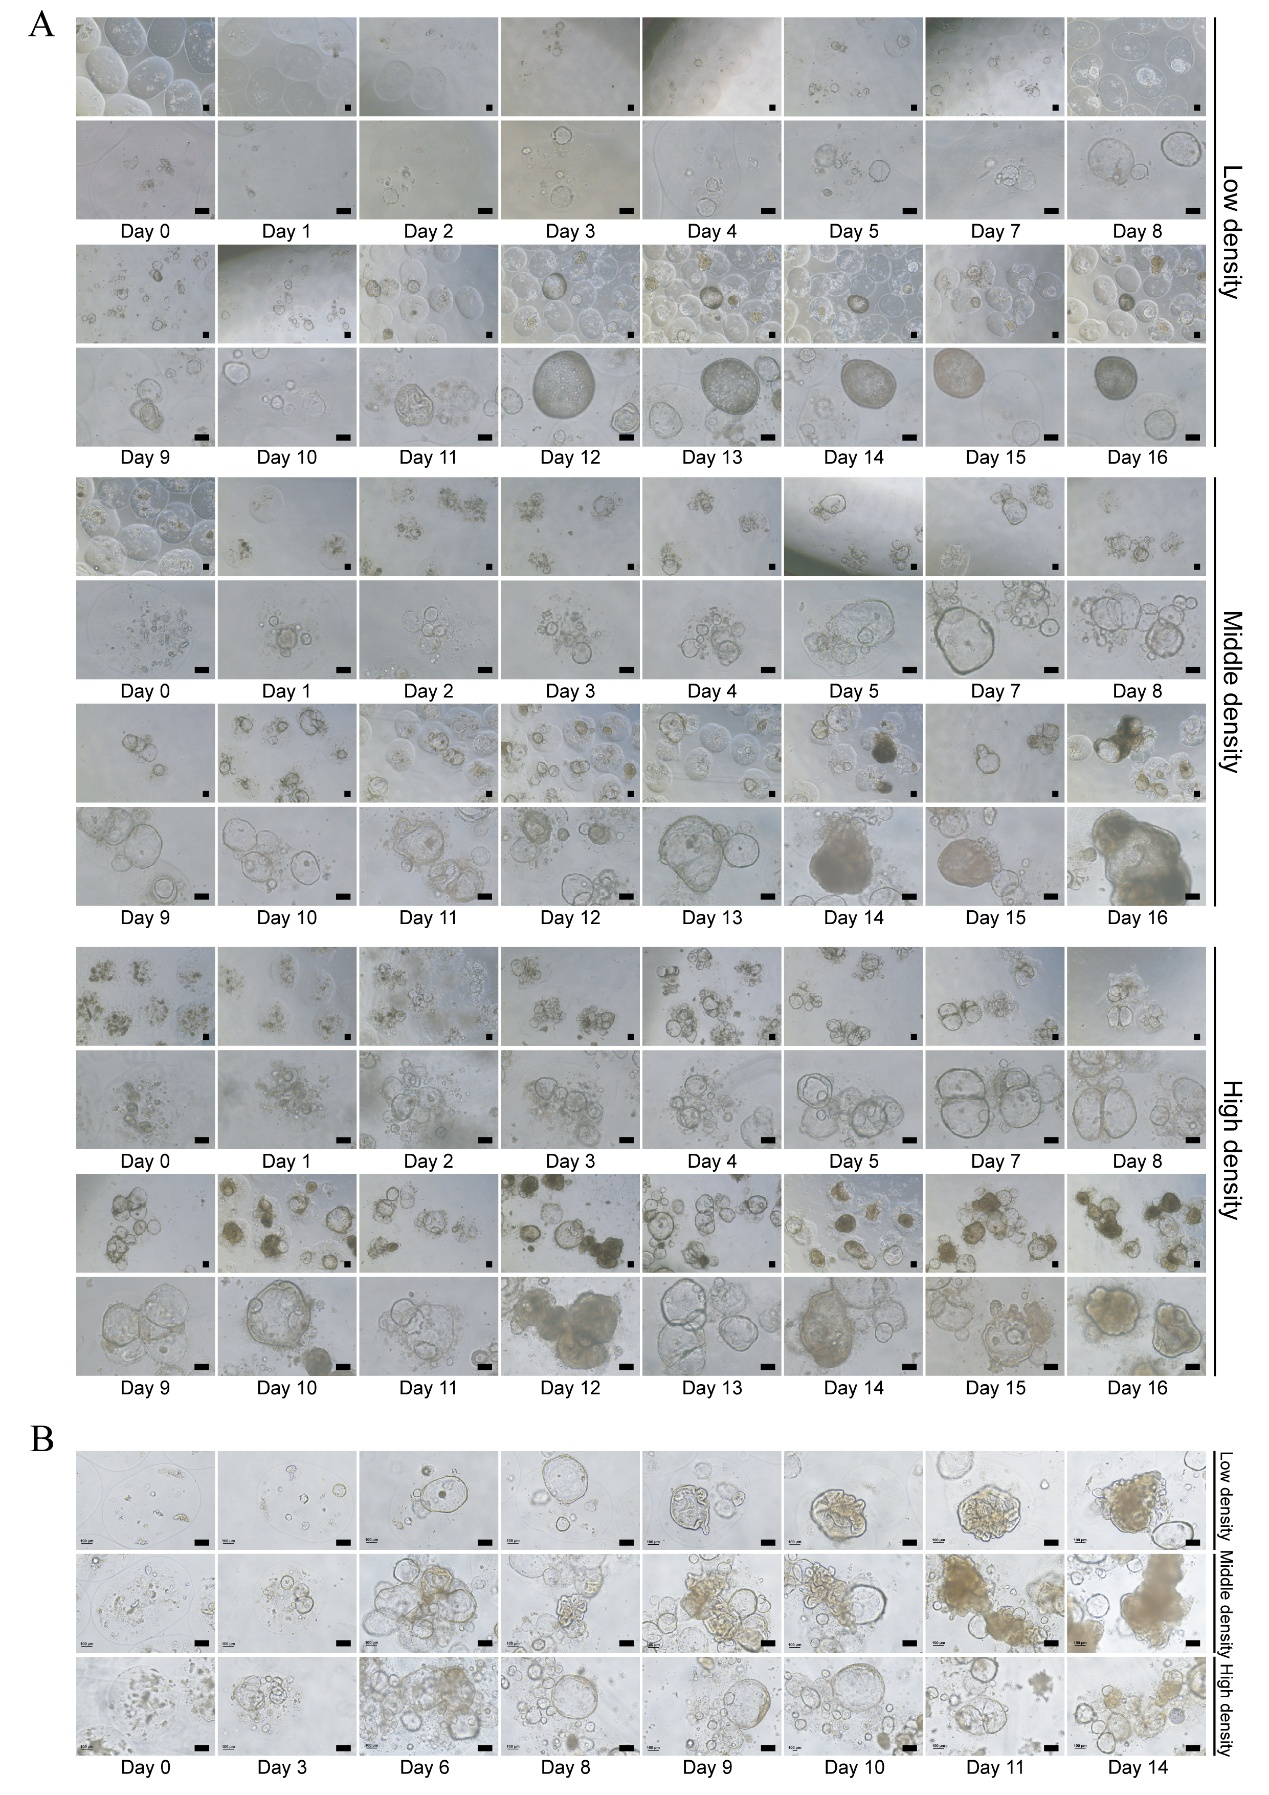
\includegraphics[width=5.45313in,height=6.39583in]{figures/sm_figure_02.png}

Figure S2 Continued growth of DEOs using low-density, middle-density, and high-density crypt suspensions. Representative images were captured from day 0 to day16. Scale bars are 100 μm.

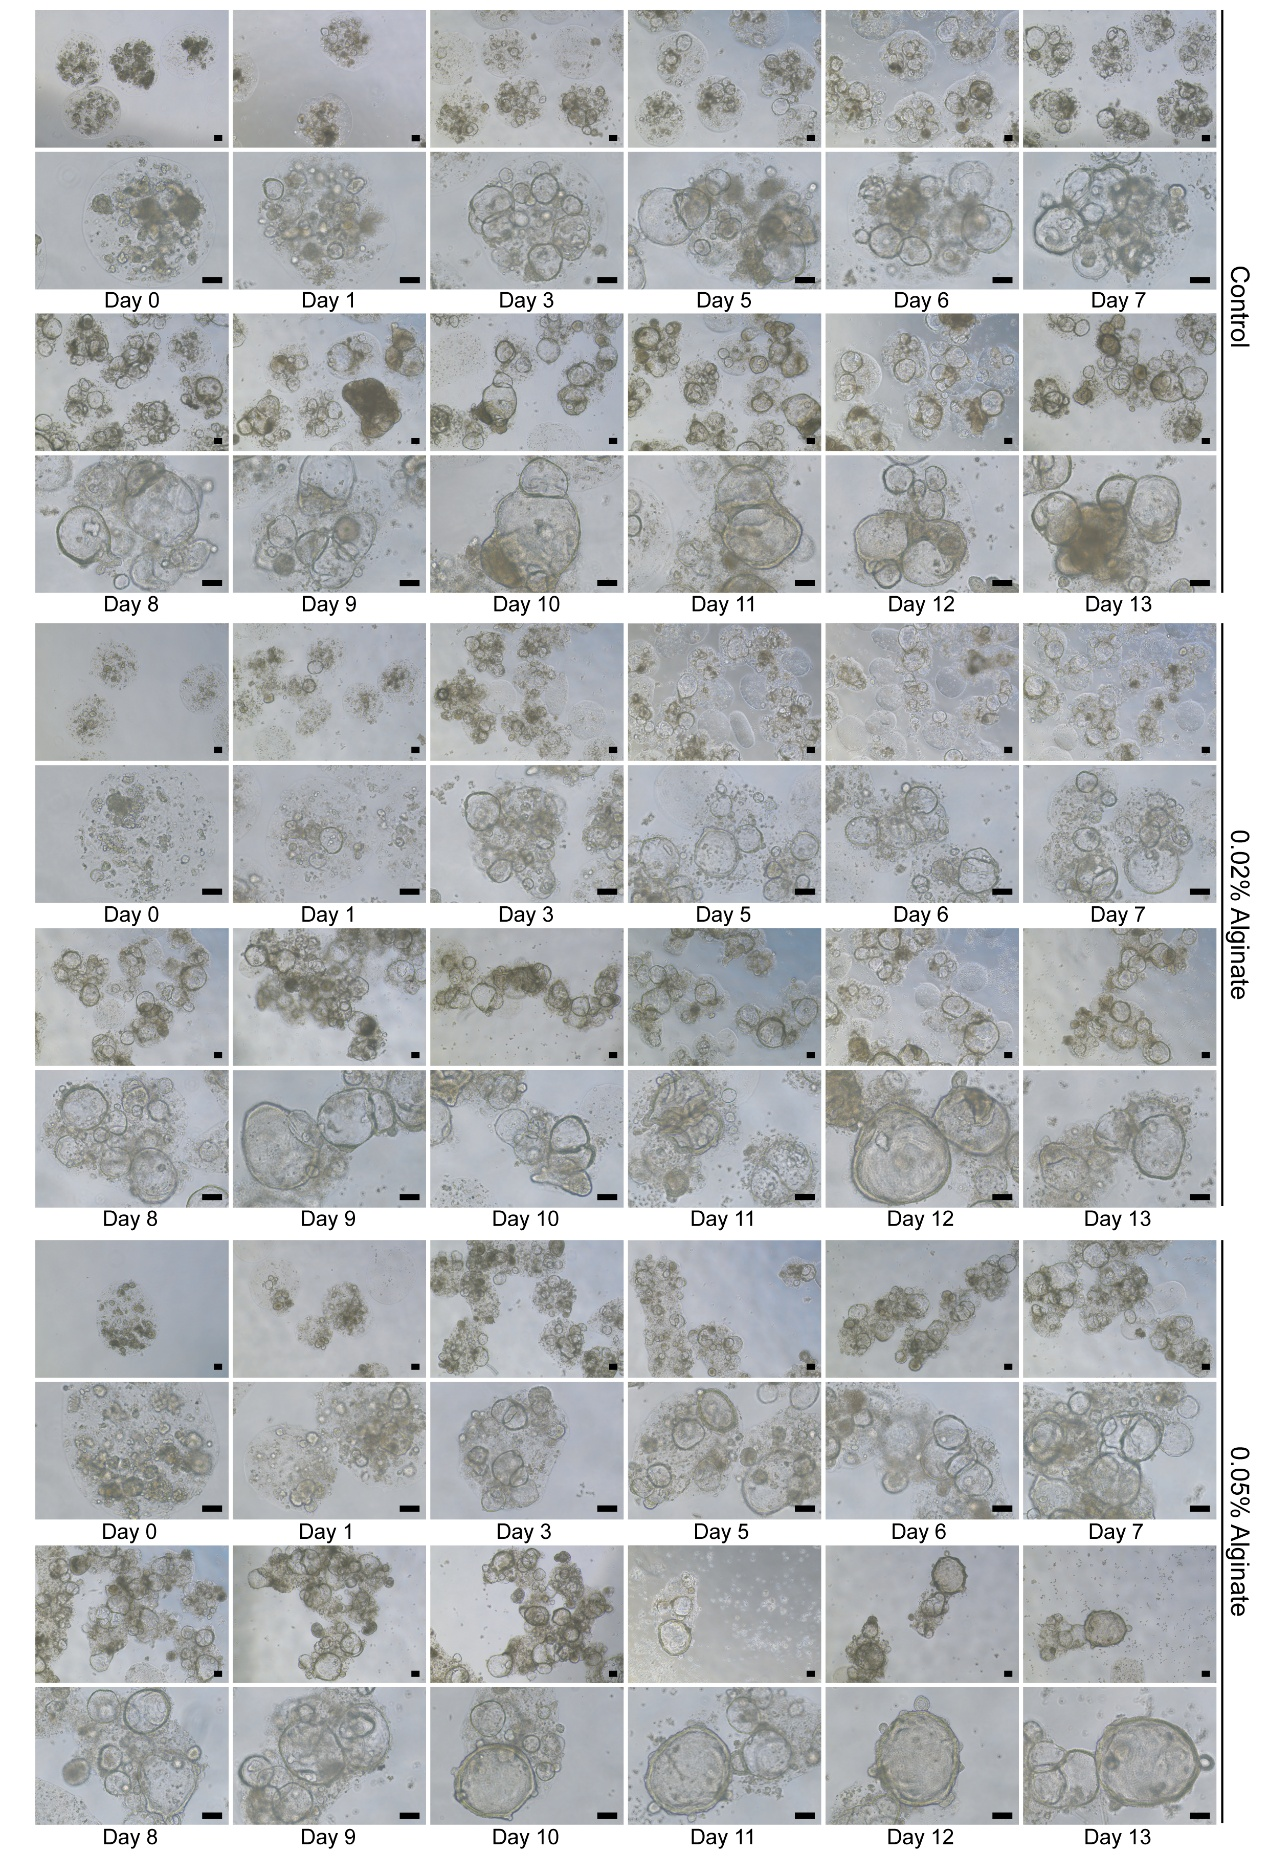
\includegraphics[width=5.76806in,height=8.51389in]{figures/sm_figure_03.png}

Figure S3 Alginate incorporation of droplet-engineered organoids. DEOs in Matrigel alone (control) or Matrigel adding sodium alginate at final concentrations of 0.02\% (low alginate) or 0.05\% (high alginate). Representative images were captured from day 0 to day 13. Scale bars are 100 μm.

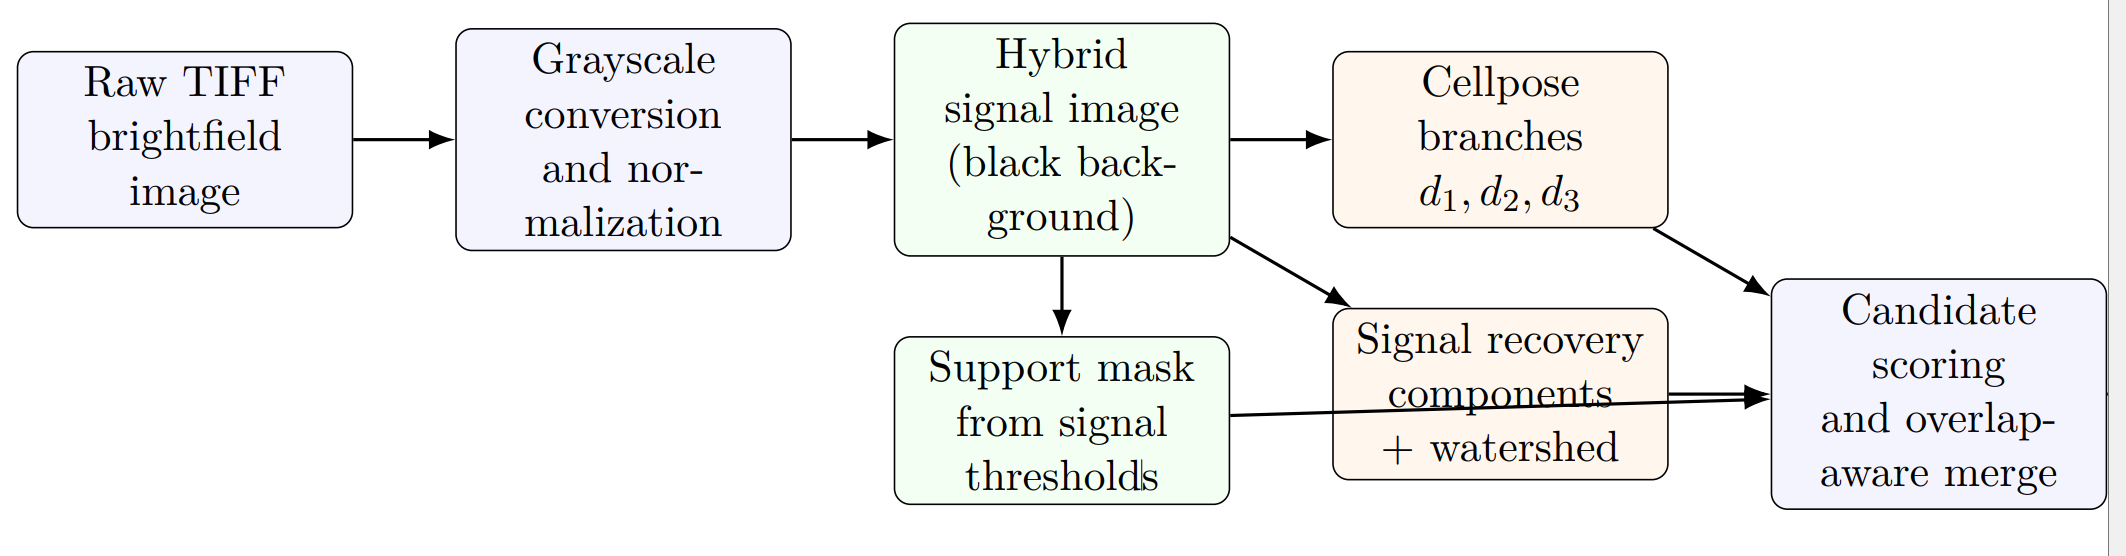
\includegraphics[width=5.76806in,height=1.50833in]{figures/sm_figure_04.png}

\sout{Figure S4 DEO segmentation workflow}

\sout{The segmentation workflow generated final instance label maps from brightfield images using hybrid signal preprocessing, multiscale Cellpose branches, and signal-based large-mass recovery, followed by overlap-aware merging of candidate objects}

（重新做一个好看的放正文）

\textbf{Figure S4 Representative segmentation outputs for density experiments}

\textbf{Figure S5 Representative segmentation outputs for alginate experiments}

\textbf{Figure S6 Representative segmentation outputs for Y-27632 experiments}

Table S1

\begingroup
\scriptsize
\setlength{\tabcolsep}{1pt}
\begin{longtable}[]{@{}>{\raggedright\arraybackslash}p{0.50in}>{\raggedright\arraybackslash}p{0.65in}>{\raggedright\arraybackslash}p{0.72in}>{\raggedright\arraybackslash}p{0.82in}>{\raggedright\arraybackslash}p{1.55in}@{}}
\toprule
& \shortstack{\textbf{Growth}\\\textbf{metric}} & \shortstack{\textbf{Differentiation}\\\textbf{metric}} & \textbf{Fusion metric} & \textbf{Rationale} \\
\midrule
\endhead
\textbf{Density} & Total segmented area & Organoid darkness P90 & Peripheral-to-central internal edge ratio & Total area is the main segmentation-based growth proxy. Darkness P90 captures darker, more differentiated morphologies. The peripheral-to-central ratio reflects redistribution of edge structure from the organoid periphery toward the interior during fusion. \\
\textbf{Alginate} & Average perimeter & Wall darkness P90 & Peripheral-to-central internal edge ratio & Average perimeter provides a morphology-sensitive readout of organoid expansion. Wall darkness P90 captures darker, thickened epithelial walls associated with differentiation. The same fusion metric was used because it reports the relative shift of edge signal from peripheral regions to the interior. \\
\textbf{Y-27632} & Mean organoid area (derived from segmented instance areas) & Organoid darkness P90 & Center-weighted edge sum & Mean organoid area summarizes organoid size while reducing confounding from fusion-related changes in object number. Darkness P90 captures differentiation-associated darkening. The center-weighted edge sum emphasizes interior edge structure and is therefore sensitive to fusion-associated structural integration. \\
\bottomrule
\end{longtable}
\endgroup

Abbreviations: P90, 90th percentile; DEO, droplet-engineered organoid.

Source Data 1. Statistical analysis of density experiments at matched time points

Source Data 2. Pairwise statistical comparisons between density groups and control at matched time points

Source Data 3. Statistical analysis of alginate experiments at matched time points

Source Data 4. Pairwise statistical comparisons between alginate groups and control at matched time points

Source Data 5. Statistical analysis of Y-27632 experiments at matched time points

Source Data 6. Pairwise statistical comparisons between Y-27632 groups and control at matched time points

\textbf{SI References}

{[}1{]}

{[}2{]}

\end{document}
